\chapter{TASK\_1.}

\textbf{Цель работы:}

\begin{itemize} 
	\item Создать сервер;
	\item Работа с POST запросами;
	\item Работа с GET запросами;
	\item Работа с CSS.
\end{itemize}

\textbf{Задание 1}

Создать сервер. Сервер должен выдавать страницу с тремя текстовыми полями и кнопкой. В поля ввода вбивается информация о почте, фамилии и номере телефона человека. При нажатии на кнопку "Отправить" введённая информация должна отправляться с помощью POST запроса на сервер и добавляться к концу файла (в файле накапливается информация). При этом на стороне сервера должна происходить проверка: являются ли почта и телефон уникальными. Если они уникальны, то идёт добавление информации в файл. В противном случае добавление не происходит. При отправке ответа с сервера клиенту должно приходить сообщение с информацией о результате добавления (добавилось или не добавилось). Результат операции должен отображаться на странице.

\textbf{Задание 2}

Добавить серверу возможность отправлять клиенту ещё одну страницу. На данной странице должно быть поле ввода и кнопка. В поле ввода вводится почта человека. При нажатии на кнопку "Отправить" на сервер отправляется GET запрос. Сервер в ответ на GET запрос должен отправить информацию о человеке с данной почтой в формате JSON или сообщение об отсутствии человека с данной почтой.

\textbf{Задание 3}

Оформить внешний вид созданных страниц с помощью CSS. Информация со стилями CSS для каждой страницы должна храниться в отдельном файле. Стили CSS должны быть подключены к страницам.

\begin{lstlisting}[caption=Код программы. TASK\_1. Главнвая функция main]
	
\end{lstlisting}

\begin{lstlisting}[caption=Код программы. TASK\_1. Реализация заданий]
	
\end{lstlisting}


\textbf{Вывод:}

\begin{itemize} 
	\item Был создан сервер;
	\item Была реализована работа с POST запросами;
	\item Была реализована работа с GET запросами;
	\item Была реализована работа с CSS.
\end{itemize}

\textbf{Пример работы:}

% \begin{figure}[ht!]
% 	\centering{
% 		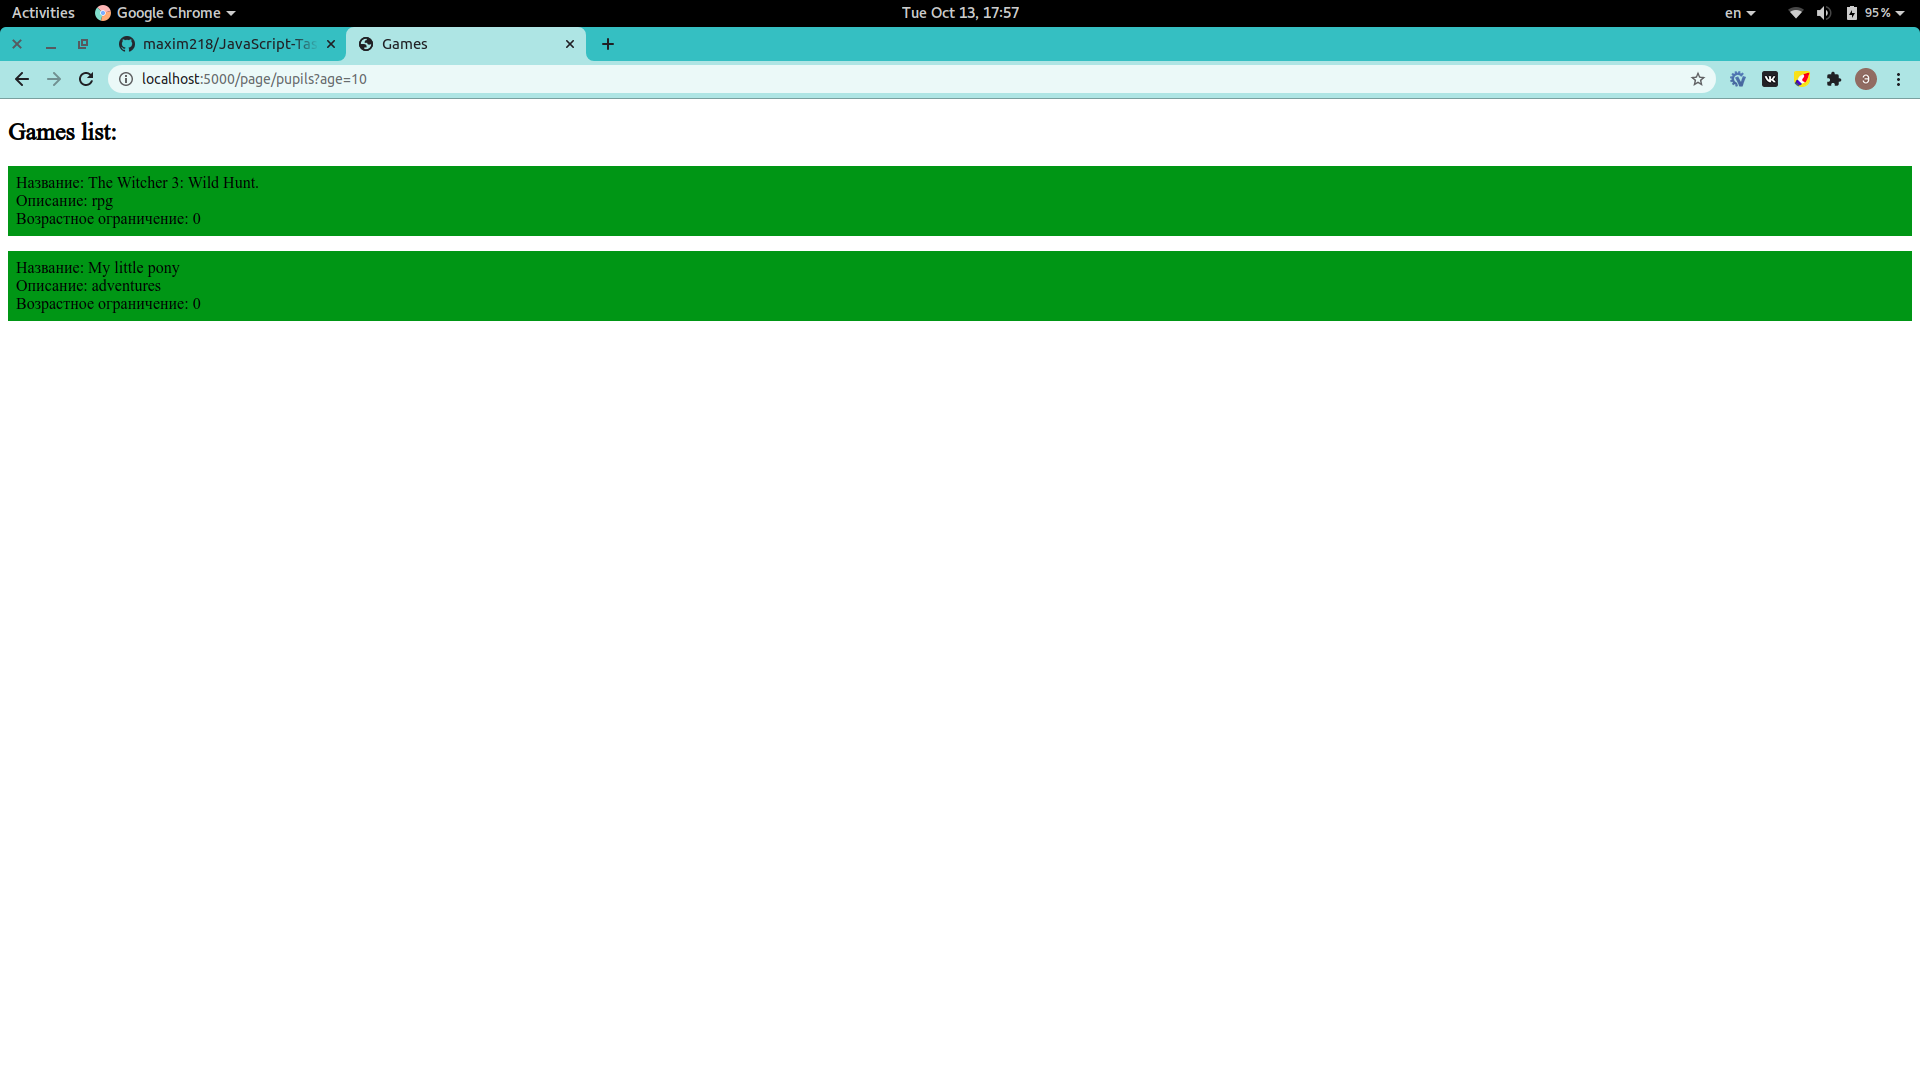
\includegraphics[width=0.9\textwidth]{img/1.png}
% 		\caption{Пример работы программы}}
% \end{figure}


\chapter{TASK\_2.}

\textbf{Цель работы:}

\begin{itemize} 
	\item Создать сервер.
	\item Реализовать страницу с использованием шаблонизатора.
	\item Изучить и реализовать работу с cookie.
\end{itemize}

\textbf{Задание 1}

Создать сервер. В оперативной памяти на стороне сервера создать массив, в котором хранится информация о компьютерных играх (название игры, описание игры, возрастные ограничения). Создать страницу с помощью шаблонизатора. В url передаётся параметр возраст (целое число). Необходимо отображать на этой странице только те игры, у которых возрастное ограничение меньше, чем переданное в url значение.

\textbf{Задание 2}

Создать сервер. В оперативной памяти на стороне сервера создать массив, в котором хранится информация о пользователях (логин, пароль, хобби, возраст). На основе cookie реализовать авторизацию пользователей. Реализовать возможность для авторизованного пользователя просматривать информацию о себе.

\begin{lstlisting}[caption=Код программы. TASK\_2. Реализация задания 1]
	"use strict";

	// Импорт библиотек.
	const express = require("express");
	// Импорт библиотеки для работы с файлами.
	const fs = require("fs");

	function main() {
		// запускаем сервер
		const app = express();
		const port = 5000;
		app.listen(port);
		console.log(`Server on port ${port}`);
	
		// Активируем шаблонизатор.
		app.set("view engine", "hbs");
	
		// Выдаем страницу с массивом игр, у которых возрастное
		// Ограничение младше, чем то, которое передано в url.
		app.get("/page/pupils", function (request, response) {
			// Получаем возраст,введенный пользователем из url.
			let age = request.query.age;
			age = parseInt(age);
			// Если корявый url пришел, сообщаем обо этом и выходим из метода.
			if (!age) {
				response.end("Age input error!");
				return
			}
	
			// Открываем файл с играми.
			const FILE_NAME = __dirname + "/game.json";
			const contentFile = fs.readFileSync(FILE_NAME, "utf-8");
			const gamesArray = JSON.parse(contentFile);
			// Создаем результирующий массив,
			// В котором будут удовлетворяющие условию игры. 
			const resultArray = [];
	
			// Пробегаемся по всем имеющимся играм.
			for (let i = 0; i < gamesArray.length; i++) {
				// Если удовлетворяет условию 
				// Добавляем в результурующий массив.
				if (gamesArray[i].age_limit < age)
					resultArray.push(gamesArray[i])
			}
			// Создаем объект, которые подставится в шаблонизатор.
			const infoObject = {
				// Описание.
				descriptionValue: "Games list:",
				// Массив игр.
				gamesArray: resultArray
			};
	
			response.render("pageGames.hbs", infoObject);
		});
	}
	
	main()
\end{lstlisting}


\begin{lstlisting}[caption=Код программы. TASK\_2. Реализация задания 2]

\end{lstlisting}

\textbf{Вывод:}

\begin{itemize} 
	\item Был создан сервер.
	\item Была реализована страница с использованием шаблонизатора.
	\item Была изучена и реализована работа с cookie.
\end{itemize}


\textbf{Пример работы:}

\begin{figure}[ht!]
	\centering{
		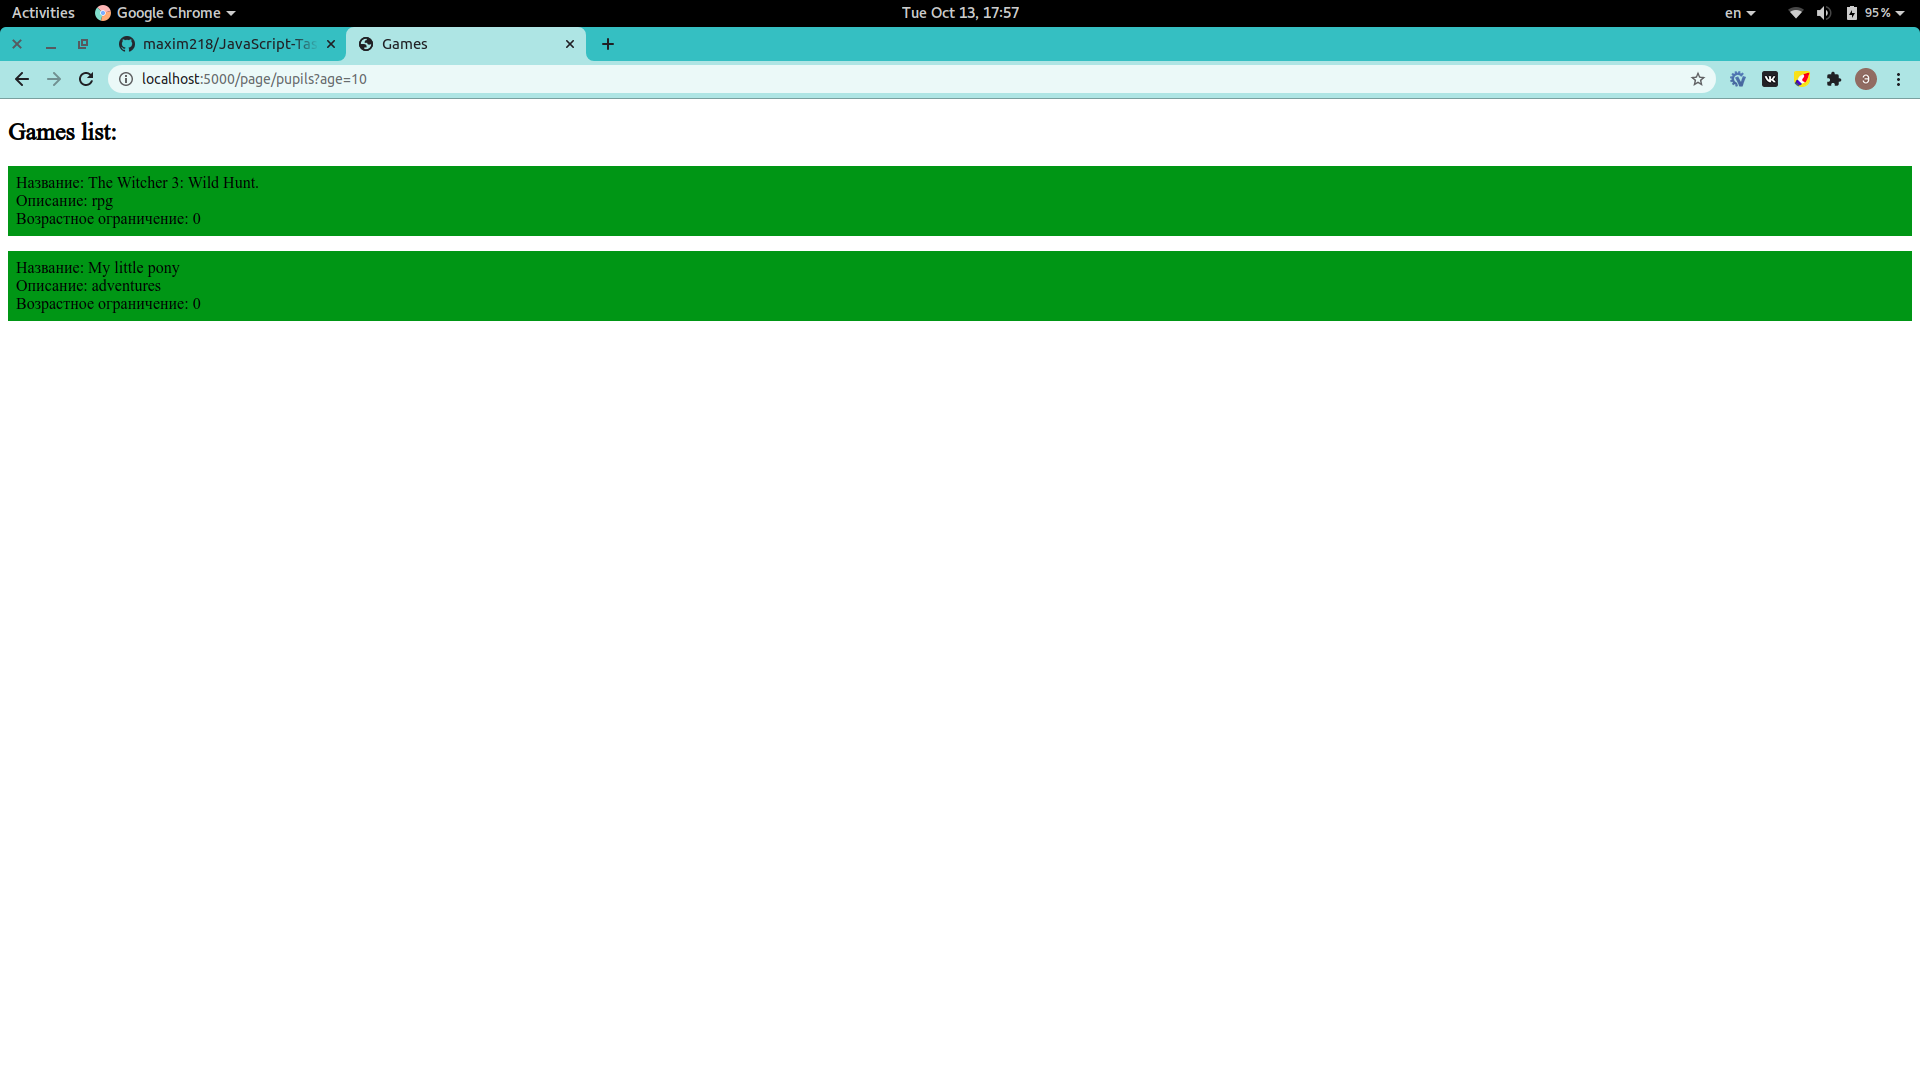
\includegraphics[width=0.9\textwidth]{img/1.png}
		\caption{Пример работы программы}}
\end{figure}

\begin{figure}[ht!]
	\centering{
		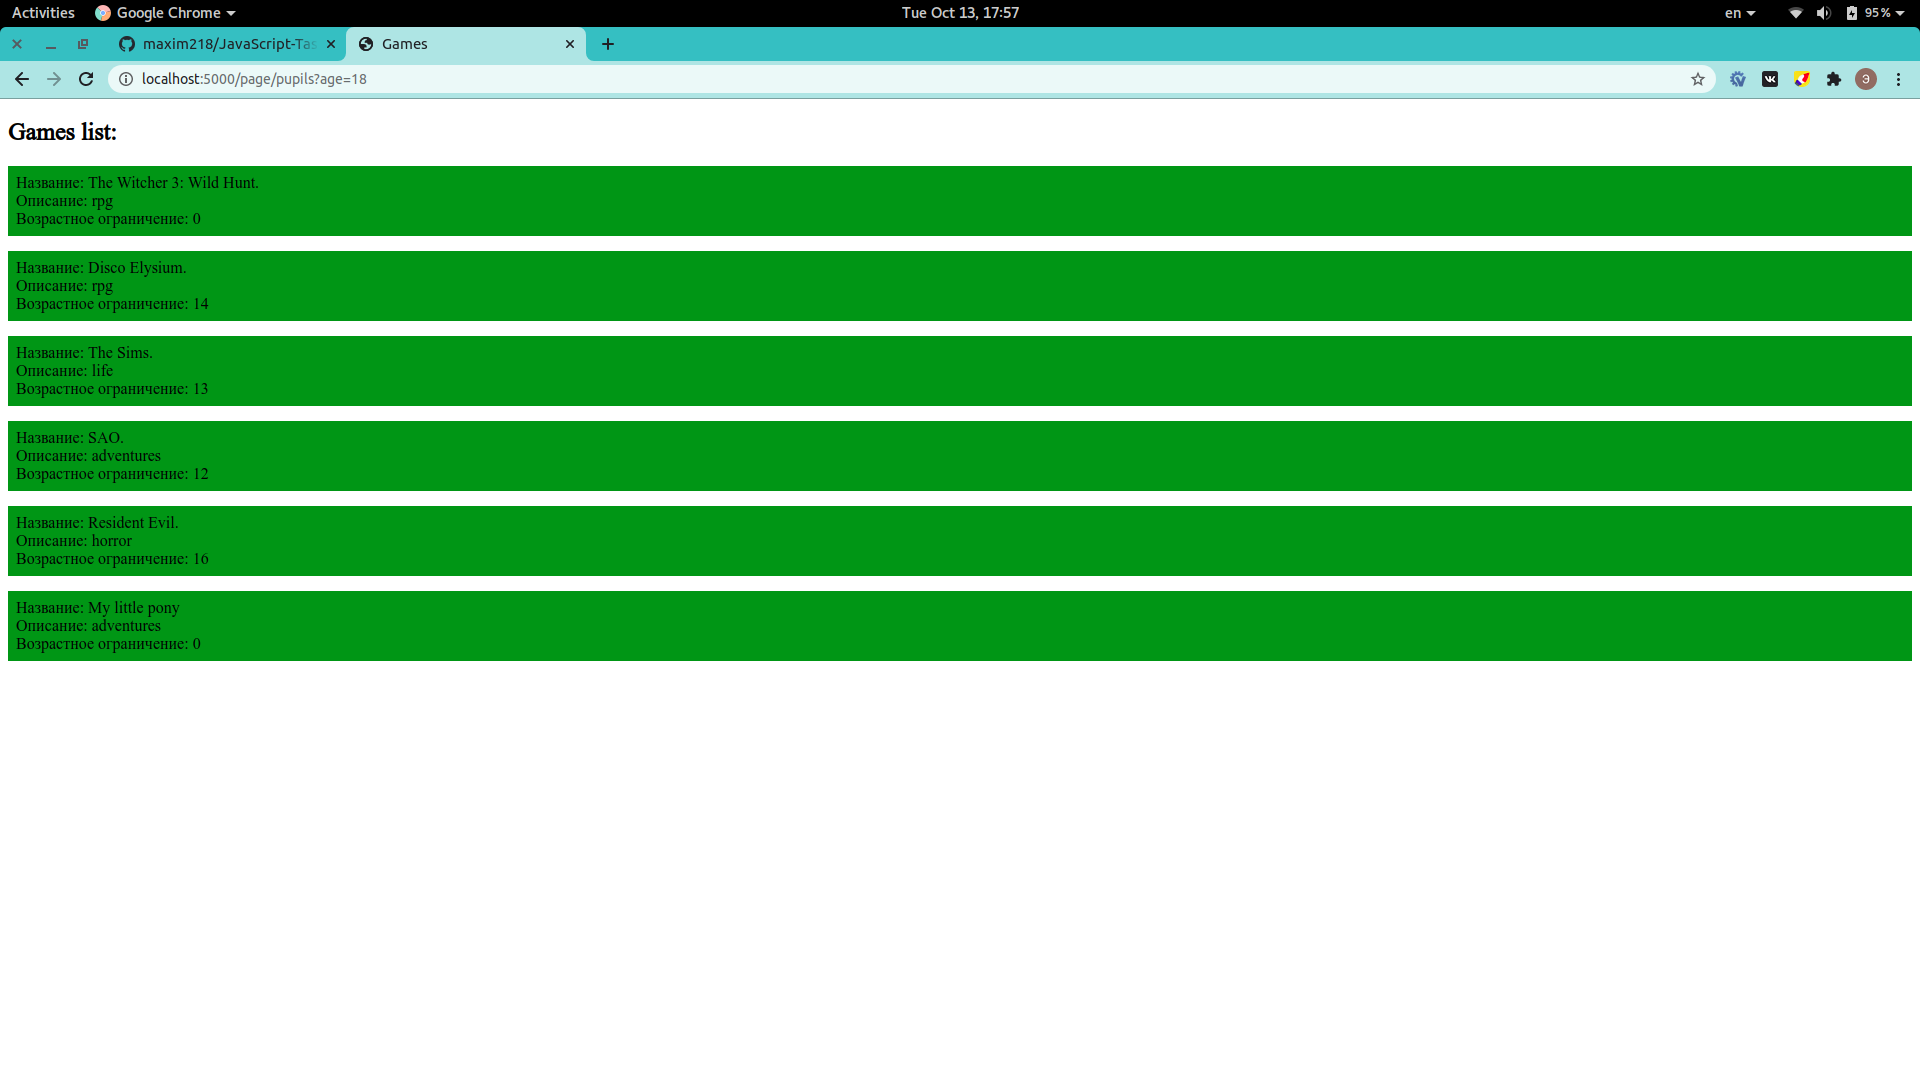
\includegraphics[width=0.9\textwidth]{img/2.png}
		\caption{Пример работы программы}}
\end{figure}
